\section{Solução proposta}

\begin{frame}		
	\begin{block}{Solução proposta}
		A solução proposta neste mestrado recomenda atividades usando três conceitos importantes na área de recomendação de atividades para \emph{workflows} científicos: %i) frequência de atividades; ii) compatibilidade entre entrada e saída; e ii) semântica de atividades
		\begin{enumerate}
			\item frequência de atividades;
			\item compatibilidade entre entrada e saída;
			\item semântica de atividades;
		\end{enumerate}
		
		
	\end{block}
\end{frame}


\begin{frame}		
	\begin{block}{Desenvolvimento da ontologia}
		A ontologia foi desenvolvida usando a metodologia \emph{Skeletal}, que contém as seguintes fases:
		\begin{enumerate}
			\item Identificar a finalidade;
			\item Construção da ontologia:
			\begin{enumerate}
				\item Captura da ontologia;
				\item Codificação da ontologia;
				\item Integração com ontologias existentes;
			\end{enumerate}
			\item Validação;
			\item Documentação.
		\end{enumerate}
	\end{block}
\end{frame}

\begin{frame}		
	\begin{block}{Ontologia desenvolvida}
		\begin{figure}
			\begin{minipage}[b]{0.3\textwidth}
				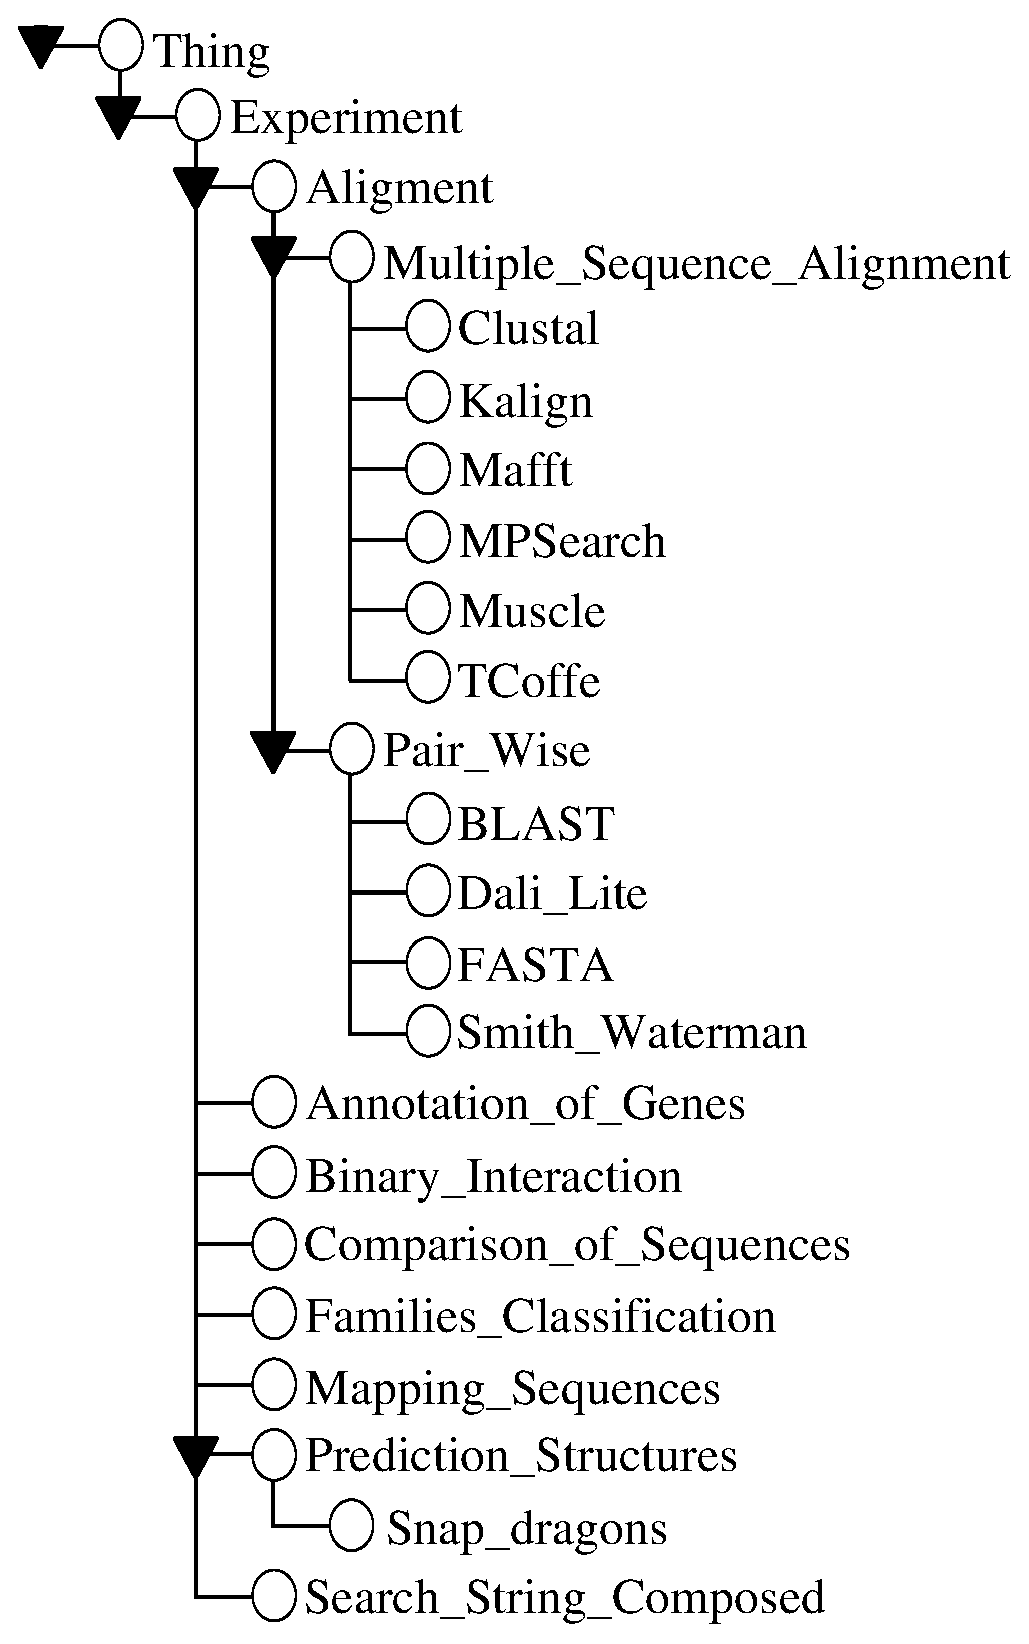
\includegraphics[width=\textwidth]{./secoes/SolucaoProposta/ontologia.eps}
				%\caption{Ontologia desenvolvida}
			\end{minipage}
		\end{figure}
	\end{block}
\end{frame}


\begin{frame}		
	\begin{block}{Matriz para técnicas da literatura}
		\begin{table}[htb]
			\centering
			\begin{tabular}{|c|c|c|c|c|}  \hline
				\textbf{\emph{Workflow}} & \textbf{Ativ \(\mathbf{01}\)} & \textbf{Ativ \(\mathbf{02}\)} & \textbf{\(\mathbf{\ldots}\)} & \textbf{Ativ \(\mathbf{280}\)}  \\ \hline
				01 			  & 1 			  & 0 			  & \(\ldots\) 	  & 0  				\\ \hline
				02 			  & 1 			  & 1 			  & \(\ldots\) 	  & 1  				\\ \hline
				03 			  & 1 			  & 0 			  & \(\ldots\) 	  & 1  				\\ \hline
				\(\vdots\) 		  			  & \(\vdots\) 	  & \(\vdots\) 	  & \(\vdots\) 	  & \(\vdots\) 		\\ \hline
				73 			  & 1 			  & 0 			  & \(\ldots\) 	  & 0  				\\ \hline
			\end{tabular}
			\caption{Matriz de entrada para técnicas da literatura correlata}
			\label{tabela_matriz_de_dados}
			%\vspace{0.1cm}
			%\source{\varAutorData}
		\end{table}
	\end{block}
\end{frame}


\begin{frame}		
	\begin{block}{Matriz para técnicas da classificação}
		\begin{table}[!htb]
			\tiny
			\centering
			\begin{tabular}{|c|c|c|c|c|c|c|c|c|}  \hline
				\textbf{\(\#\)} & \textbf{\emph{Workflow}} & \textbf{Ativ \(\mathbf{01}\)} & \textbf{Ativ \(\mathbf{02}\)} & \textbf{\(\mathbf{\ldots}\)}  & \textbf{Ativ \(\mathbf{279}\)} & \textbf{Ativ \(\mathbf{280}\)} & \textbf{Rótulo} \\ \hline
				
				1	&		01		 			   & 1 			  & 0 			  & \(\ldots\) 	  & 0 & 0  			& T	\\ \hline
				2	&		01 					   & 1 			  & 0 			  & \(\ldots\) 	  & 0 & 0  			& T	\\ \hline
				\(\vdots\)  &  \(\vdots\) 	   	   & \(\vdots\)   & \(\vdots\) 	  & \(\vdots\) 	  & \(\vdots\) & \(\vdots\) & \(\vdots\)\\ \hline
				59	&		01 					   & 1 			  & 0 			  & \(\ldots\) 	  & 0 & 0   		& T	\\ \hline
				1	&		01		 			   & 0 (removida) 		  & 1 (adicionada) &\(\ldots\)& 1 & 0	& F	\\ \hline
				2	&		01 					   & 0 (removida)& 0 		  & \(\ldots\) 	  & 1 (adicionada) & 0& F	\\ \hline
				\(\vdots\)  &		\(\vdots\) 	   & \(\vdots\) & \(\vdots\) 	  & \(\vdots\) 	  & \(\vdots\) & \(\vdots\) & \(\vdots\) \\ \hline
				59	&		01 					   & 0 (removida)			  & 0 			  & \(\ldots\) & 0 & 1 (adicionada)& F \\ \hline
				&\(\vdots\) & & & & & & 																		\\ \hline
				1	&		73		 			   & 1 			  & 1  & \(\ldots\) 	  & 0 & 0  			& T	\\ \hline
				2	&		73 					   & 1 			  & 1  & \(\ldots\) 	  & 0 & 0  			& T	\\ \hline
				\(\vdots\)  &		\(\vdots\) 	   & \(\vdots\)   & \(\vdots\) 	  & \(\vdots\) 	  & \(\vdots\) & \(\vdots\) & \(\vdots\) \\ \hline
				59	&		73 					   & 1 			  & 1  & \(\ldots\) 	  & 0 & 0   		& T	\\ \hline
				1	&		73		 			   & 1 (adicionada) & 0 (removida)  & \(\ldots\) 	  & 1 & 0   		& F	\\ \hline
				2	&		73 					   & 1 			  & 0 (removida)  & \(\ldots\)& 1 (adicionada) & 0  & F	\\ \hline
				\(\vdots\)  &		\(\vdots\) 	   & \(\vdots\)   & \(\vdots\) 	  & \(\vdots\) 	  & \(\vdots\) & \(\vdots\) & \(\vdots\)	\\ \hline
				59	&		73 					   & 1 			  & 0 (removida)  & \(\ldots\) 	  & 0 & 1 (adicionada) & F	\\ \hline
			\end{tabular}
			\caption{Exemplo de matriz de entrada para técnicas de classificação e regressão}			
			\label{tabela_matriz_de_dados_adapatada_classificacao_regressao}
			%\vspace{0.1cm}
			%\source{\varAutorData}
		\end{table}
	\end{block}
\end{frame}



\begin{frame}		
	\begin{block}{Técnica proposta}
		Para explicar a técnica proposta será usada a figura:
			\begin{figure}
				\begin{minipage}[b]{0.7\textwidth}
					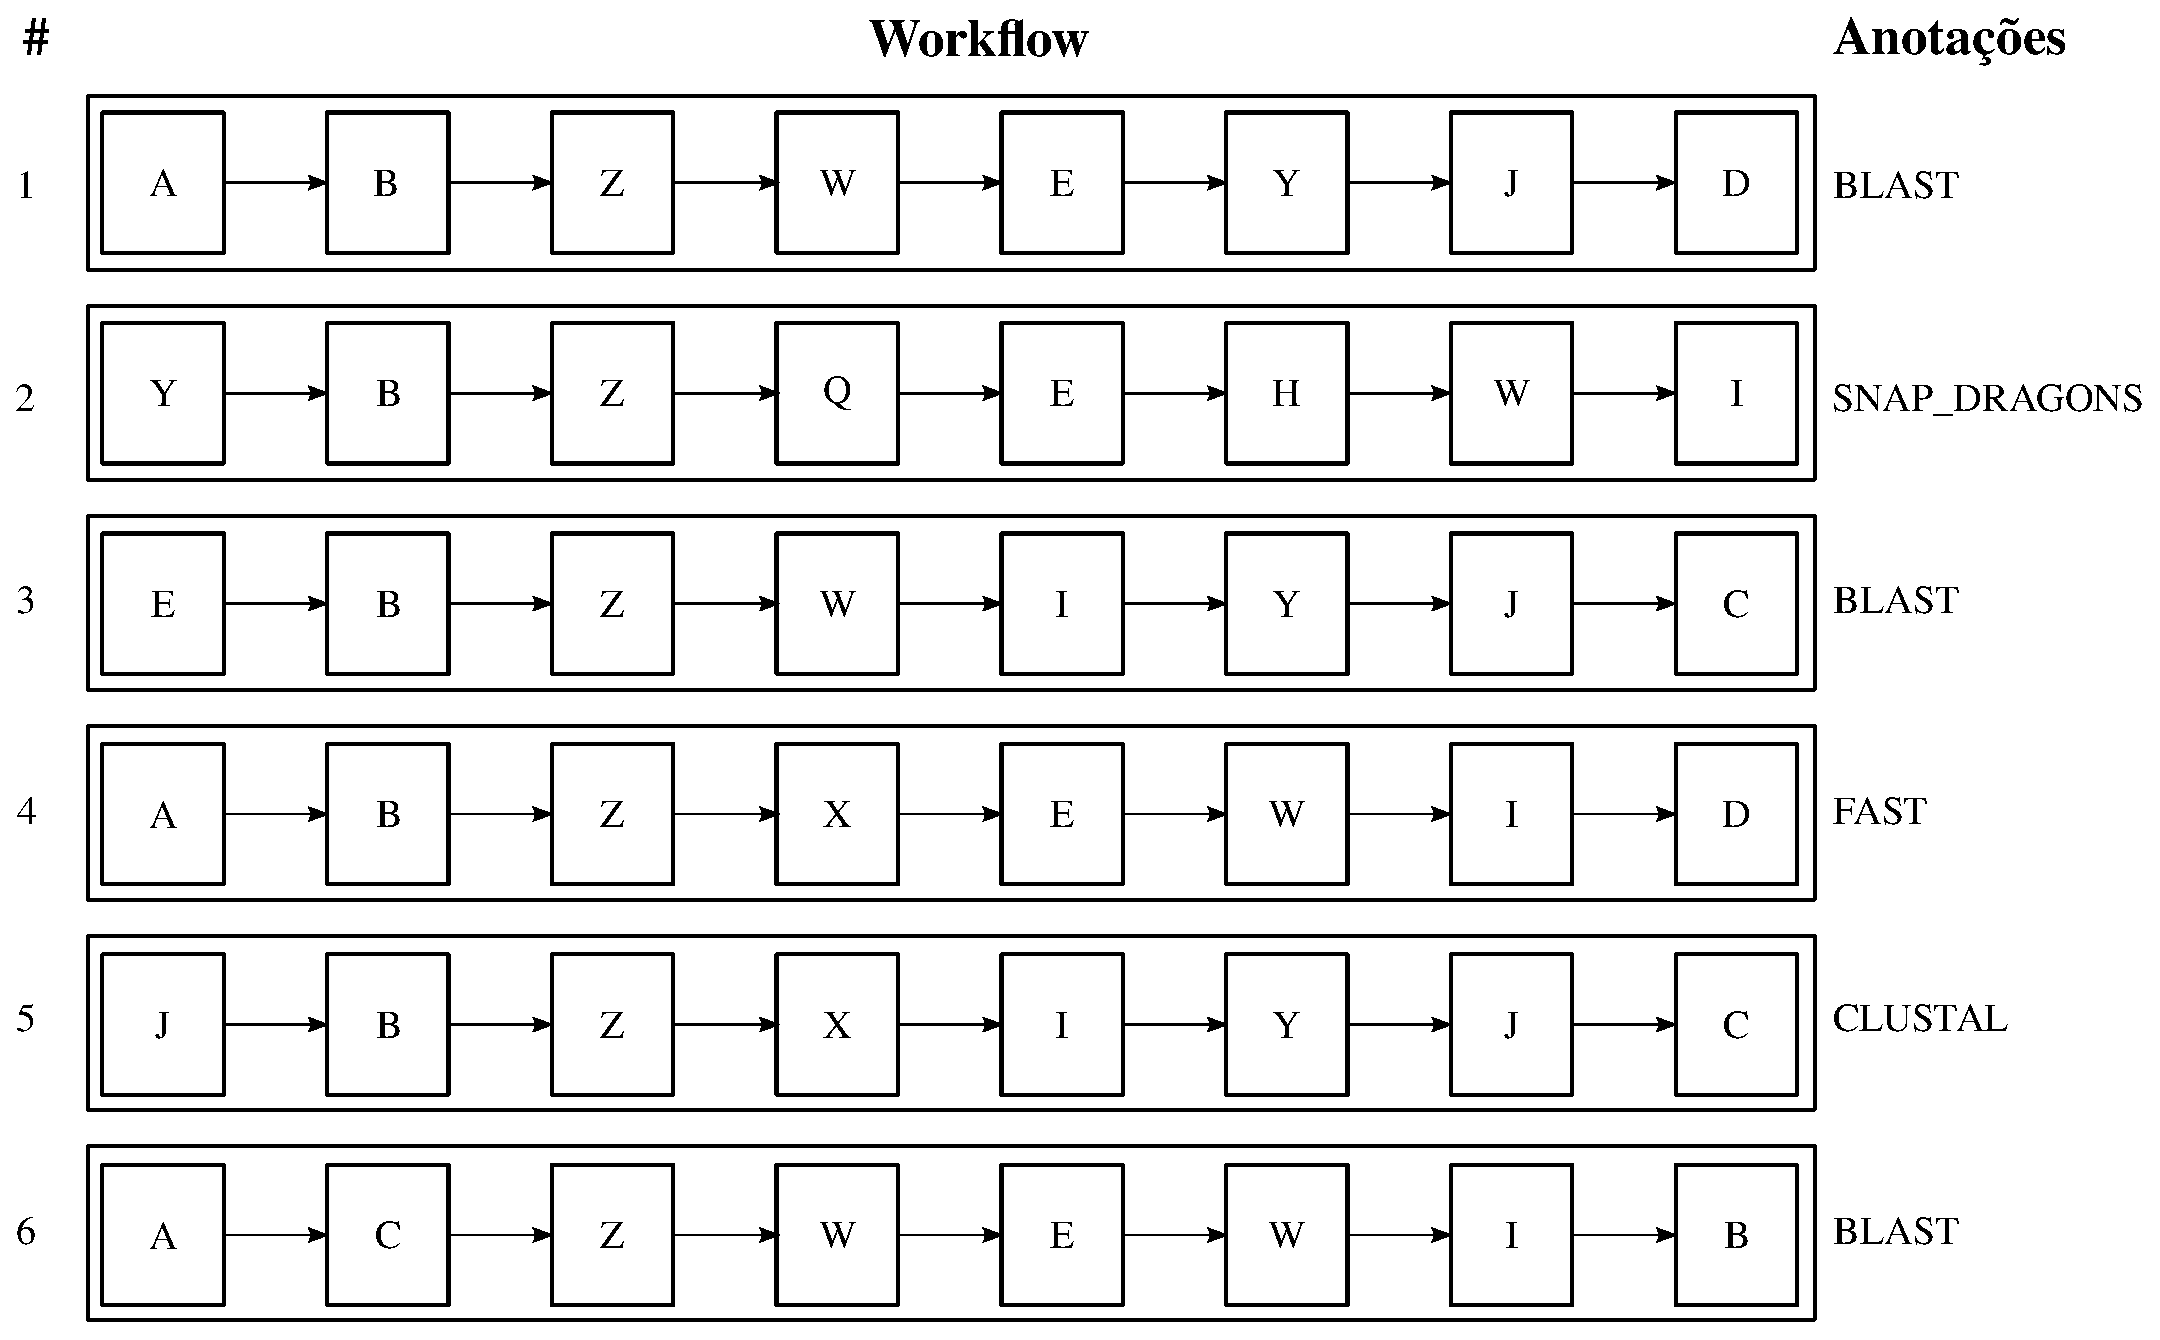
\includegraphics[width=\textwidth]{./secoes/SolucaoProposta/recomendacaofreqontologia.eps}
					\caption{Exemplo de banco de dados de \emph{workflows} científicos}
				\end{minipage}
			\end{figure}
	\end{block}
\end{frame}

%Isso eu devo falar!
%\begin{frame}		
%	\begin{block}{Técnica proposta}
%		Suponha que durante a construção do \emph{workflow} \(1\) (ver figura \ref{FIGURA_ONTOLOGIA_CONSTRUIDA}) um cientista insere a atividade \emph{Z} e solicita uma recomendação. O sistema vai procurar na lista das atividades posteriores a \emph{Z} ordenadas por frequência e conceito ontológico e irá retornar a lista de recomendação apresentada na tabela~\ref{tabela_lista_recomendacao_ordenada_frequencia}. 
%		
%		A ordenação por conceito ontológico, além de ser estável serve como critério de desempate, para o caso de duas atividades terem a mesma frequência. Neste exemplo, de acordo com a lista de recomendação da tabela~\ref{tabela_lista_recomendacao_ordenada_frequencia}, a atividade \emph{W} seria recomendada em primeiro lugar ao cientista, o que representa um acerto.
%			
%	\end{block}
%\end{frame}

\begin{frame}		
	\begin{block}{Técnica proposta}
\begin{table}[!htb]
	\centering
	\begin{tabular}{|c|c|c|c|}  \hline
		\textbf{Posição na Lista} & \textbf{Ativ} & \textbf{Frequência} & \textbf{Anotação Atividade} 	\\ \hline
		1				& W 				& 3 				& BLAST				\\ \hline
		2				& X 				& 2 				& FAST, CLUSTAL		\\ \hline
		3				& Q 				& 1 				& SNAP DRAGONS		\\ \hline
		\(\vdots\)		& \(\vdots\)		& \(\vdots\) 		& \(\vdots\)		\\ \hline
		280				& \(\vdots\)		& \(\vdots\)		& \(\vdots\)	\\ \hline
	\end{tabular}
	\caption{Recomendação para a atividade \emph{Z} ordenada por frequência e conceito ontológico}
	\label{tabela_lista_recomendacao_ordenada_frequencia}
	%\vspace{0.1cm}
	%\source{\varAutorData}
\end{table}
	\end{block}
\end{frame}

%Isso eu devo falar!
%\begin{frame}		
%	\begin{block}{Técnica proposta}
%As atividades são anotadas com a mesma anotação dos \emph{workflows} que as contém, dessa forma é possível que haja pelo menos uma atividade com mais de uma anotação. Isto gera um novo caso de recomendação a ser considerado, suponha que ambas as atividades \emph{W} e \emph{X} contenham dentro de suas listas de anotação o conceito \emph{BLAST}. Neste caso seria recomendada a atividade com menor número de anotações, por ser considerada mais específica para o experimento em questão. Caso ambas as atividades tenham o mesmo número de anotações é utilizada a ordem alfabética de conceitos como critério de desempate. Se ocorrer um novo empate é usado um seletor aleatório.
%	\end{block}
%\end{frame}
